\vspace{-4pt}
\begin{sectionbox}
\section{Parallel Programming}
\subsection{Parallelism}\smallskip
Syntax best explained by example: 
\end{sectionbox}
\vspace{-4pt}
\begin{lstlisting}[language=C++]
#include <iostream>
#include <vector>
#include <algorithm>
#include <thread>
#include <cassert>
#include <cmath>

// PRE:  [begin, end) must be a valid interval.
// POST: Returns the sum of the values in [begin, end).
template <typename It, typename T = typename It::value_type>
void sum_seq(It begin, It end, T& result) {
  T sum = 0;
  
  for (It curr = begin; curr != end; ++curr)
    sum += *curr;
    
  result = sum;
}

// PRE:  [begin, end) must be a valid interval.
// PRE:  0 < max_threads
// POST: Returns the sum of the values in [begin, end), 
//       using at most max_threads threads.
template <typename It, typename T = typename It::value_type>
double sum_par(
    const It begin, 
    const It end, 
    unsigned max_threads)
{
  assert(0 < max_threads);
  
  // Prevents corner cases further down
  if (begin == end) return 0; 
  
  // Using more threads than there are values to sum up would 
  // yield a partition size of zero
  unsigned thread_count = std::min(
      (unsigned)(end - begin), max_threads);
  assert(thread_count != 0); // Should not happen

  std::vector<std::thread> threads; // Stores forked threads
  // Partial sums
  std::vector<double> partial_sums(thread_count, 0);

  // Summation will be parallelised by (conceptually) split-
  // ting the input interval into thread_count partitions
  unsigned partition_size = (end - begin) / thread_count;
  assert(partition_size != 0); // Should not happen
  
  It partition_begin = begin;

  // Fork sequential sum computations
  for (unsigned i = 0; i < thread_count - 1; ++i) {
    It partition_end = partition_begin + partition_size;
    
    auto worker = std::thread(
      [=,&partial_sums] () {
        T t;
        sum_seq(partition_begin, partition_end,t);
        partial_sums[i] = t;
      }
      
      );

    threads.push_back(std::move(worker));

    // The current chunk's end is the next chunk's begin
    partition_begin = partition_end;
  }
  
  auto worker = std::thread(
            sum_seq<It, double>, 
            partition_begin, 
            end, 
            std::ref(partial_sums[partial_sums.size() - 1]));

  threads.push_back(std::move(worker));

  // Iterate over the forked threads and wait for each thread 
  // to finish
  for (auto& td : threads)
    td.join();

  // As a last step we have to sum up the partial sums that 
  // the forked threadscomputed. We could parallelise this as 
  // well, but since partial_sums istypically a small vector, 
  // we sum it up sequentally.
  double result = 0;
  sum_seq(partial_sums.begin(), partial_sums.end(), result);
  
  return result;
}
\end{lstlisting}

\vspace{-4pt}
\begin{sectionbox}
\subsection{Concurrency}\smallskip
\textbf{Important Concepts}\par\smallskip
\begin{itemize}
    \item Nondeterministic Thread Scheduling: The scheduler can interrupt (pause) any thread at virtually any moment, to schedule another one
    \item $\Rightarrow$ multiple threads are executed in a \textbf{non-deterministic order}, and many different thread-interleavings are possible
    \item A program has a \textbf{race condition} if, during any possible execution with the same inputs, its observable behaviour (results, output, ...) can change if events happen in different order
    \item A program has a \textbf{data race} if, during any possible execution, a memory location could be written from one thread, while concurrently being read or written from another thread
\end{itemize}

\textbf{Options for Preventing Bad Interleavings}
\begin{enumerate}
    \item Share only immutable data (if possible)
    \item Use atomic data types (if possible)
    \item Use mutual exclusion to make arbitrary code atomic
\end{enumerate}
\end{sectionbox}
\vspace{-4pt}
\begin{sectionbox}
\textbf{Mutual Exclusion}
\begin{itemize}
    \item C++ provides \lstinline{std::mutex} with \lstinline{.lock()} and \lstinline{.unlock()} for protecting sensitive code-regions.
    \item A \textbf{deadlock} is a situation in which the overall program cannot make any progress, because each thread waits for another thread to finish its action.
    \begin{enumerate}
        \item Establish a strict total order between the shared resources
        \item Ensure that the resources are always acquired according to this order
    \end{enumerate}
\end{itemize}
\end{sectionbox}
\vspace{-4pt}
\begin{sectionbox}
\textbf{Lock Guards}
Guard automatically locks mutex - and more importantly, also unlocks it at the end of the scope of the guard.

Different locks exist:
\begin{itemize}
    \item \lstinline{std::lock_guard}: basic lock for single mutex
    \item \lstinline{std::scoped_lock}: multiple mutexes, prevents deadlocks (if used exclusively)
    \item \lstinline{std::unique_lock}: single mutex, more control (e.g. when mutex is locked)
    \item \lstinline{std::shared_lock}: for reader-writer situations
    
    \begin{itemize}
        \item Many threads only read the shared data in their critical section
        \item Few threads write the shared data
        \item Reading in parallel is fine, but writers need exclusive access
        \item Example: shared phonebook; much more often read than updated
    \end{itemize}
\end{itemize}

\begin{center}
  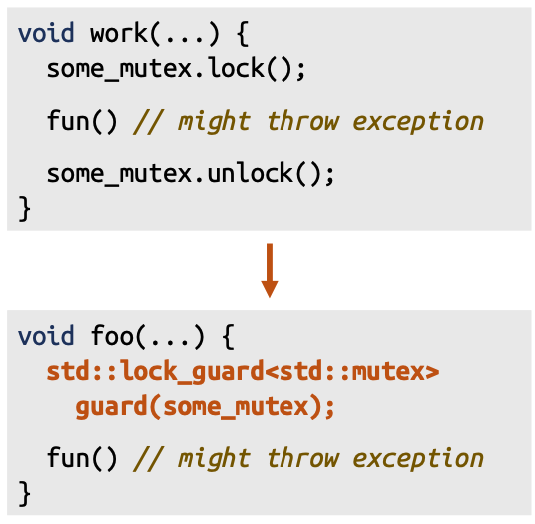
\includegraphics[width=0.5 \columnwidth]{img/LockGuard.png}
\end{center}
\end{sectionbox}